\documentclass[a4paper,10pt,twoside]{article}
%%%%%%%%%%% Packages %%%%%%%%%%
\usepackage[margin=1in]{geometry}
\usepackage{amsmath, amssymb,mathtools}
\usepackage{fancyhdr}
\usepackage{sectsty}
\usepackage{graphicx,wrapfig}
\usepackage{enumitem}
\usepackage{float}
\usepackage{braket}
\usepackage{bbm}
\usepackage{tikz,calc}

%%%%%%%%%%% Macros %%%%%%%%%%
\def \note#1 {\vspace{-1em}\paragraph{\bfseries #1}}
\def \dd {{\rm d}}
\def \id {{\mathbbm{1}}}
\def \order {\mathcal{O}}
\def\bquad{\mkern-18mu}
\DeclareMathOperator{\trace}{tr}
\DeclareMathOperator{\spanset}{span}

%%%%%%%%%%% Tikz Definitions %%%%%%%%%%
\usetikzlibrary{shapes, arrows,positioning,fit}
\tikzstyle{plain} = [draw,thick,circle,inner sep=0,minimum size=0.5cm,font=\footnotesize]
\tikzstyle{mps} = [draw,thick,rectangle,rounded corners=.1cm,inner sep=0,minimum size=0.5cm]
\tikzstyle{mpo} = [draw,thick,circle,inner sep=0,minimum size=0.5cm]
\tikzstyle{diagonal} = [draw,thick,diamond,inner sep=0,minimum size=0.5cm]
\tikzstyle{index} = [-,thick,font=\footnotesize]
\tikzstyle{virtual} = [-,thick,dotted,font=\footnotesize]
\tikzstyle{site} = [draw,solid,circle,minimum size=2pt,inner sep=0pt,outer sep=0pt,fill=black]

\def \tu {0.25cm}

%%%%%%%%%%% Formatting %%%%%%%%%%
\pagestyle{fancy}
\renewcommand{\footrulewidth}{0.5pt}

\fancyhf{}
\lhead{29/07/2017}
\chead{Quantum Information Methods in Many-Body Physics}
\rhead{PH2269}
\lfoot{Giacomo Giudice~~~~giacomo.giudice@mpq.mpg.de}
\rfoot{Page \thepage}

\allsectionsfont{\normalfont\sffamily}

%%%%%%%%%%% Here Begins Document %%%%%%%%%%
\begin{document}
\title{\vspace{-1cm}\sffamily Solutions to Homework 8\vspace{-1cm}}
\author{}
\date{}
\maketitle
\thispagestyle{fancy}

\begin{section}{}
Expanding to first order, we obtain the Lie--Trotter approximation 
\[
  U(\tau) = U_1(\tau) \, U_2(\tau) + \order \left( \tau^2 \right) .
\]
The second-order expansion is
\begin{align*}
  e^{-i H_1 \tau/2} e^{-i\tau H_2} e^{-iH_1\tau/2} 
  &= \exp \left( -i \frac{\tau}{2} H_1 -i \tau H_2 - \frac{\tau^2}{4}[H_1,H_2] \right) \exp\left( -i\frac{\tau}{2}H_2 \right) + \order(\tau^3)  \\
  &= \exp \left( -i \tau H_1 -i \tau H_2 - \frac{\tau^2}{4} \big( [H_1,H_2]  + [H_2,H_1]\big) \right) + \order(\tau^3)    \\
  &= U(\tau) + \order(\tau^3)\,.
\end{align*}
Higher-order formulas require applying repeatedly many operators to an MPS.
This will make its bond dimension increase exponentially quickly, making it challenging to go to large bond dimensions.
On the other hand, truncating after each application of a partial evolution operator will keep the bond dimension small, but will introduce more truncation errors. 
 If the truncation errors are significant, this will render a high-order decomposition useless since we will not be cancelling out the terms that the decomposition tries to remove.
\end{section}

\begin{section}{}
The procedure to compress a bond can be understood through the canonization procedure.
In order to gauge a generic MPS tensor $A^{\sigma}_{a,b}$ in a left- or right-canonical form, one employs the SVD decomposition of the matrix $A_{(\sigma,a)(b)}$ or $A_{(a)(\sigma,b)}$, as shown below.
The steps are: (a) reshaping, (b) SVD decomposition, (c) reshaping of one matrix and contracting of the other two with the next element.
\begin{figure}[H]
  \begin{center}
    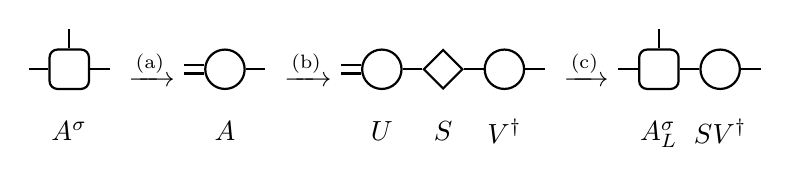
\begin{tikzpicture}[auto, node distance=\tu]
      \node[mps]  (m) {};
      \node[below=of m] {$\vphantom{|} A^{\sigma}$};
      \draw[index] (m.west) -- +(-\tu,0);
      \draw[index] (m.north) -- +(0,\tu);
      \draw[index] (m.east) -- +(\tu,0);
      \node[right=of m] (eq0) {~$\xrightarrow[]{{\rm (a)}}$~};
      \node[plain,right=of eq0]  (m1) {};
      \node[below=of m1] {$\vphantom{|} A$};
      \draw[index] ([yshift=-1.5pt]m1.west) -- +(-\tu,0);
      \draw[index] ([yshift=1.5pt]m1.west) -- +(-\tu,0);
      \draw[index] (m1.east) -- +(\tu,0);
      \node[right=of m1] (eq1) {~$\xrightarrow[]{{\rm (b)}}$~};
      \node[plain,right=of eq1]  (u1) {};
      \node[diagonal,right=of u1]  (s1) {};
      \node[plain,right=of s1]  (v1) {};
      \node[below=of u1] {$\vphantom{|} U$};
      \node[below=of s1] {$\vphantom{|} S$};
      \node[below=of v1] {$\vphantom{|} V^\dag$};
      \draw[index] ([yshift=-1.5pt]u1.west) -- +(-\tu,0);
      \draw[index] ([yshift=1.5pt]u1.west) -- +(-\tu,0);
      \draw[index] (v1.east) -- +(\tu,0);
      \draw[index] (u1.east) -- (s1.west);
      \draw[index] (s1.east) -- (v1.west);
      \node[right=of v1] (eq2) {~$\xrightarrow[]{{\rm (c)}}$~};
      \node[mps,right=of eq2]  (m2) {};
      \node[plain,right=of m2]  (sv) {};
      \draw[index] (m2.west) -- +(-\tu,0);
      \draw[index] (m2.north) -- +(0,\tu);
      \draw[index] (m2.east) -- (sv.west);
      \draw[index] (sv.east) -- +(\tu,0);
      \node[below=of m2] {$\vphantom{|} A_L^{\sigma}$};
      \node[below=of sv] {$\vphantom{|} SV^\dag$};
    \end{tikzpicture}
    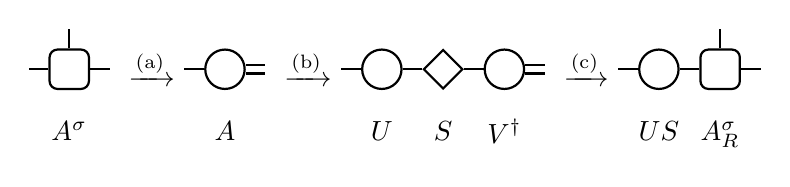
\begin{tikzpicture}[auto, node distance=\tu]
      \node[mps]  (m) {};
      \node[below=of m] {$\vphantom{|} A^{\sigma}$};
      \draw[index] (m.west) -- +(-\tu,0);
      \draw[index] (m.north) -- +(0,\tu);
      \draw[index] (m.east) -- +(\tu,0);
      \node[right=of m] (eq0) {~$\xrightarrow[]{{\rm (a)}}$~};
      \node[plain,right=of eq0]  (m1) {};
      \node[below=of m1] {$\vphantom{|} A$};
      \draw[index] (m1.west) -- +(-\tu,0);
      \draw[index] ([yshift=-1.5pt]m1.east) -- +(\tu,0);
      \draw[index] ([yshift=1.5pt]m1.east) -- +(\tu,0);
      \node[right=of m1] (eq1) {~$\xrightarrow[]{{\rm (b)}}$~};
      \node[plain,right=of eq1]  (u1) {};
      \node[diagonal,right=of u1]  (s1) {};
      \node[plain,right=of s1]  (v1) {};
      \node[below=of u1] {$\vphantom{|} U$};
      \node[below=of s1] {$\vphantom{|} S$};
      \node[below=of v1] {$\vphantom{|} V^\dag$};
      \draw[index] (u1.west) -- +(-\tu,0);
      \draw[index] (u1.east) -- (s1.west);
      \draw[index] (s1.east) -- (v1.west);
      \draw[index] ([yshift=-1.5pt]v1.east) -- +(\tu,0);
      \draw[index] ([yshift=1.5pt]v1.east) -- +(\tu,0);
      \node[right=of v1] (eq2) {~$\xrightarrow[]{{\rm (c)}}$~};
      \node[plain,right=of eq2]  (us) {};
      \node[mps,right=of us]  (m2) {};
      \draw[index] (m2.east) -- +(\tu,0);
      \draw[index] (m2.north) -- +(0,\tu);
      \draw[index] (m2.west) -- (us.east);
      \draw[index] (us.west) -- +(-\tu,0);
      \node[below=of m2] {$\vphantom{|} A_R^{\sigma}$};
      \node[below=of us] {$\vphantom{|} US$};
    \end{tikzpicture}
  \end{center}
\end{figure}
Choosing a gauge such that all tensors left of $A$ are left-canonized, and all tensors to the right are right-canonized, the overlap reduces to 
\begin{figure}[H]
  \centerline{
    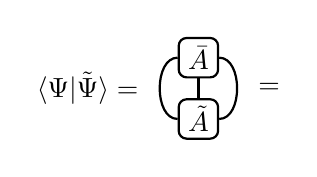
\begin{tikzpicture}[auto, node distance=\tu]
      \node[mps] (mconj) {$\bar{A}$};
      \node[mps,below=of mconj] (m) {$\tilde{A}$};
      \draw[index] (m.east) to[in=0,out=0] (mconj.east);
      \draw[index] (m.west) to[in=180,out=180] (mconj.west); 
      \draw[index] (m.north) -- (mconj.south);
      \node[fit=(m)(mconj)] (f) {};
      \node[left=of f] (overlap) {$\braket{\Psi|\tilde{\Psi}}=$};
      \node[right=of f] (eq) {$=$};
    \end{tikzpicture}
    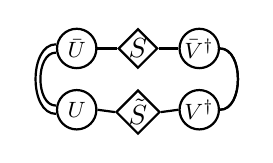
\begin{tikzpicture}[auto, node distance=\tu]
      \node[plain] (uconj) {$\bar{U}$};
      \node[diagonal,right=of uconj] (sconj) {$S$};
      \node[plain,right=of sconj] (vconj) {$\bar{V}^\dag$};
      \node[plain,below=of uconj] (u) {$U$};
      \node[diagonal,below=of sconj] (s) {$\tilde{S}$};
      \node[plain,below=of vconj] (v) {$V^\dag$};
      \draw[index] (u.east) -- (s.west);
      \draw[index] (s.east) -- (v.west);
      \draw[index] (uconj.east) -- (sconj.west);
      \draw[index] (sconj.east) -- (vconj.west);
      \draw[index] (v.east) to[in=0,out=0] (vconj.east);
      \draw[index] (v.east) to[in=0,out=0] (vconj.east);
      \draw[index] ([yshift=-1.5pt]u.west) to[in=180,out=180] ([yshift=+1.5pt]uconj.west); 
      \draw[index] ([yshift=+1.5pt]u.west) to[in=180,out=180] ([yshift=-1.5pt]uconj.west); 
    \end{tikzpicture}
    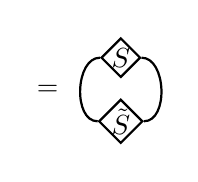
\begin{tikzpicture}[auto, node distance=\tu]
      \node[diagonal] (sconj) {$S$};
      \node[diagonal,below=of sconj] (s) {$\tilde{S}$};
      \draw[index] (s.east) to[in=0,out=0] (sconj.east);
      \draw[index] (s.west) to[in=180,out=180] (sconj.west); 
      \node[fit=(s)(sconj)] (f) {};
      \node[left=of f] (eq) {$=$};
    \end{tikzpicture}
  }
\end{figure}
Physically, from this picture it is clear that the square of the singular values correspond to the Schmidt coefficients.
We can then trim down the corresponding matrices knowing that we are discarding the smallest Schmidt coefficients, since the error is given by the sum of the square of the discarded singular values, $\| \ket{\Psi} - \ket{\tilde{\Psi}} \|^2 = \| \Psi \|^2 - \braket{\Psi|\tilde{\Psi}} - \braket{\tilde{\Psi}|\Psi} +  \| \tilde{\Psi} \|^2 = 1 - \trace\tilde{S}^2 $.
\end{section}

\begin{section}{}
No solution is presented for this exercise.
\end{section}
\end{document}
%%%%%%%%%%% Here Ends Document %%%%%%%%%%
